\documentclass[a4paper]{book}

\usepackage[a4paper, left=1in, right=1in, bottom=1in, top=0.75in]{geometry}
\usepackage[utf8]{inputenc} % input encoding for interpreter
\usepackage[T1]{fontenc}
\usepackage{amssymb}
\usepackage{newtxtext}
\usepackage{multicol}
\usepackage[newfloat]{minted}
\usepackage{graphicx}
\usepackage[italicdiff]{physics}
\usepackage{float}
\usepackage{amsmath}
\usepackage{titlepic}
\usepackage{titlesec}
\usepackage{hyperref}
\usepackage{pgfplots}
\usepackage{multirow}
\usepackage{caption}
\usepackage{subfigure}

\newenvironment{code}{\captionsetup{type=listing}}{}
\SetupFloatingEnvironment{listing}{name=Source Code}

\pgfplotsset{compat=1.18}

\graphicspath{{images/}}
\setcounter{secnumdepth}{0}
\newcommand{\srcfolder}{../firmware/src/}
\newcommand{\simfolder}{../firmware/sim/}

\titleformat{\chapter}[display]
  {\normalfont\bfseries}{}{0pt}{\Huge}
  
\title{VHDL design of a simple RISC-V architecture}
\author{Mirco Tollardo 217918}
\date{a.y. 2024-2025}


\begin{document}
\frontmatter
\maketitle

\tableofcontents

\let\cleardoublepage\clearpage
\mainmatter
\chapter{Introduction}
This document is going to describe a basic RISC-V datapath written in VHDL, starting from a simple non-pipelined architecture just to implement more complex features and instructions with a bottom-up approach.
When talking about RISC-V it is necessary to distinguish the two faces of the ISA:
\begin{itemize}
    \item \emph{Unpriviledged ISA}: that defines the user-level instruction types, which mainly compose a program to be executed.
    \item \emph{Priviledged ISA}: which defines exception management and operation modes (supervisor, hypervisor and user mode), interrupt handling and multiple other functionalities for operating system support.
\end{itemize}
The project will focus on partially implementing the base user-level instructions, defined in the unpriviledged ISA, defining at each stage of the execution what information in an instruction are used and how they affect the state of the sequential network, helping the explanation with behavioral simulations, and building the project in a way that can be later expanded with other features.
Thus, the first stage of this project will focus on implementing a datapath that executes some commands included in the User Instruction Set, in particular, for the first part of the project, the 32-bit Base Integer Instruction Set (RV32I).
The report will be divided into chapters for each of the following 5 stages of the CPU:
\begin{itemize}
\item \textbf{Instruction Fetch}
\item \textbf{Instruction Decode} 
\item \textbf{Instruction Execute} 
\item \textbf{Data Memory}
\item \textbf{Writeback} 
\end{itemize}
The completion of the first rudimental architecture, able to execute one instruction per clock cycle, has to be then optimized by introducting registers between each block, and thus achieving a \emph{pipelined architecture}, adding more complexity overall yet incrementing the performance of the circuit.\\
Once again, adding feature with a good base to start from should be easy, and the project could take another step further; One good feature is adding the capability for the processor to execute multiplications and divisions between integers, easy enough since VHDL introduces the synthetizable operators '*' and '/'.\\
One thing that won't be easy, though, is implementing floating-point operations, since it would require the introduction to a data type that follow the IEEE 754 standard for floating point numbers. The only way to avoid the problem would be having them encoded in VHDL using the data type \textbf{real}, which is not synthetizable, although it would make a good option for HDL designs that won't go further from simulation.\\
With this being said, the project will follow said procedure, while making available the code in Appendix A.


\chapter{Building an RV32I datapath}
\section{Basic Instruction Fetch}
\begin{figure}[ht!]
  \centering
  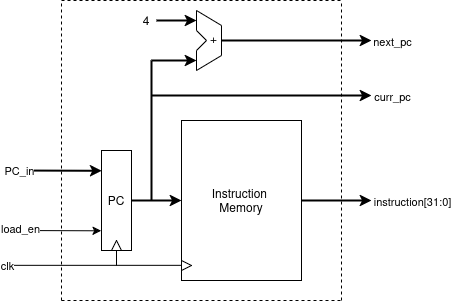
\includegraphics[scale = 0.4]{IF_BD.png}
  \caption{Basic instruction fetch block diagram}
  \label{fig:IF_BD}
\end{figure}
\subsection{Basic decription}
This stage of the datapath fetches the instruction to be executed, which is stored in the Instruction Memory. This memory can be implemented using Vivado's Block Memory Generator IP, configured as a single-port RAM with a 32-bit read-write width. The memory size should be addressable using at least 12 bits, because the AUIPC instruction must be able to load absolute addresses that are shifted by that amount into the Program Counter (PC).
The Program Counter is a register that holds the address of the current instruction and, during program execution, the latter is incremented at each rising edge of the clock; Since memory is byte-addressable and each instruction is 4 bytes long, the PC is incremented by 4 at each step. 
In this project, however, the Instruction Memory is simulated using a RAM with 32-bit words per address; While the architecture should still work with bytes, the increment is going to remain 4, but the two least significant bits of the address shall be unused from now on.
To handle jumps or branches in the program, the PC may accept another value as input from a different stage along the datapath, allowing it to be loaded with a new address after such instructions are executed.
In VHDL, a register can be synthesized by declaring a clock-dependent (and in this case also \emph{load{\_}en} dependent) \emph{signal}, hence the PC will be implemented with this method.
A VHDL entity that describes this stage can be defined as follows:\\
\begin{minted}[fontsize=\footnotesize]{vhdl}
entity instr_fetch is
 port ( 
  clk        : in std_logic;
  pc_load_en : in std_logic;
  pc_in      : in std_logic_vector(11 downto 0);

  next_pc    : out std_logic_vector(11 downto 0);
  curr_pc    : out std_logic_vector(11 downto 0);
  instr      : out std_logic_vector(31 downto 0)
  );
end instr_fetch;
\end{minted}
\vspace{1\baselineskip}
With the previously specified settings, the IP used for the Instruction Memory will generate a component that can be instantiated in the architecture as follows:\\
\begin{minted}[fontsize=\footnotesize]{vhdl}
component instruction_memory
 port(
  clka  : in std_logic;
  wea   : in std_logic;
  addra : in std_logic_vector(9 downto 0);
  dina  : in std_logic_vector(31 downto 0);
  douta : out std_logic_vector(31 downto 0));
end component;
\end{minted}
\vspace{1\baselineskip}

The inputs \emph{wea} (i.e. the write-enabling input) and \emph{dina} (data input) will be pulled low since there is no need for the moment to write inside the memory. 
Since the PC has to act as a pointer for the instruction, its output will be routed to the \emph{addra} input, excluding the first two least significant bits in order to proceed 32 bits (the length of a standard instruction) at a time.
With this being said, the only thing that is left to do is a clock-sensitive process that increments the PC or loads another address from the outside if the load-enable input of its register is pulled high. 
By implementing the register as a \emph{signal} named \emph{pc{\_}reg}, the resulting VHDL script for the architecture is shown in Source Code \ref{code:IF_code}.


\subsection{Simulation}
A testbench for this simulation will require the PC to be incremented by 4 so that every location in the memory is addressed, but in order to actually see a stream of instructions at the output a .coe file for the initialization of the instruction memory is required:

\begin{minted}{text}
  memory_initialization_radix=16;
  memory_initialization_vector=
  00000293,     --> addi x5, x0, 0
  00100313,     --> addi x6, x0, 1
  005303B3;     --> add x7, x6, x5
\end{minted}
A .coe file requires the hexadecimal dump of the program, in this given example each instruction has its assembly equivalent on the right.\\
For the testbench, a simple clock can be simulated with a process while a small register can be simulated for storing \emph{next{\_}pc} and re-routing its value on \emph{pc{\_}in}, hence the testbench, shown in Code \ref{code:IF_TB} gives the resulting behavior:

\begin{figure}[h!]
  \centering
  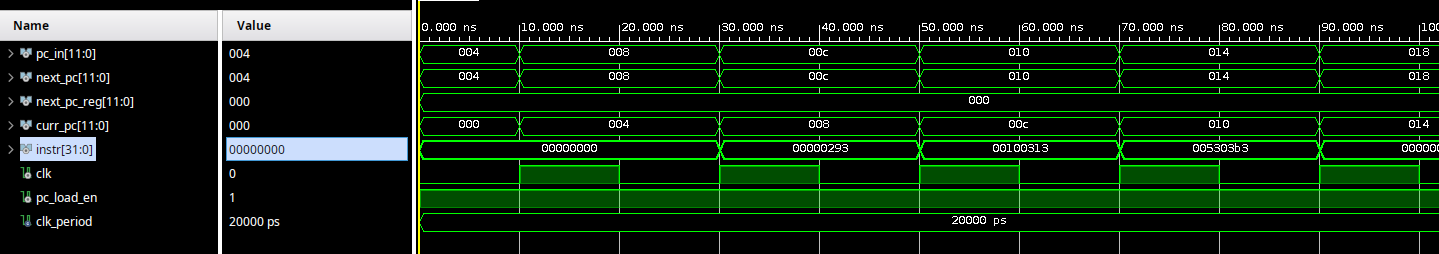
\includegraphics[scale = 0.45]{IF_sim.png}
\end{figure}

The results state that \emph{curr{\_}pc}, in fact, acts as a register, refreshed as the clock's rising edge approaches, and the flow of instructions are the same as the ones stated in the \emph{.coe} file. 


\section{Basic Instruction Decode}
\begin{figure}[ht!]
  \centering
  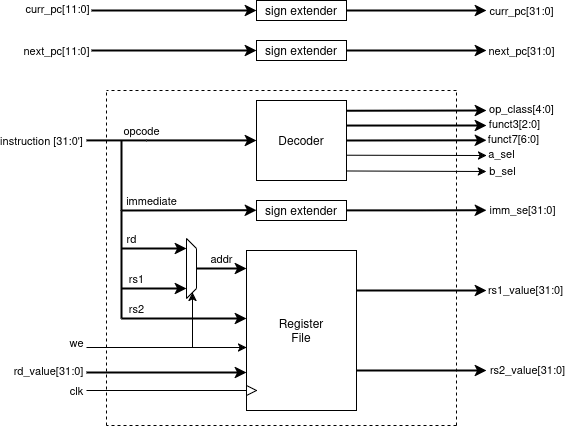
\includegraphics[scale=0.4]{ID_BD.png}
  \caption{A block diagram for the instruction decoding stage}
  \label{fig:ID_BD}
\end{figure}

\subsection{Instruction formats}
After an instruction is returned from the fetching stage, it must be decoded in order to select the right action that has to be performed in the next step of the datapath. The RISC-V ISA provides instructions for register to operate with other registers, constants, with the data memory or the PC itself.
In the base ISA, there are four core instruction formats:
\begin{itemize}
\item \textbf{R-type}: Register to register instructions. These instructions are expected to use two registers as sorce for data to be elaborated and then store the result of the operation in a destination register. This instruction has to select the two sources as operands for the next stage to treat them as such, hence two boolean outputs \emph{a\_sel} and \emph{b\_sel} will be pulled high to indicate that the registers pointed by the values of rs1 (bits 19 down to 15) and rs2 (bits 24 down to 20) are used as operands.
\item \textbf{I-type}: Immediate instructions. The value stored in rs1 (bits 19 to 15) and an immediate value (bits 31 to 20) make the operands of the operation to be executed. \emph{a\_sel} has to be set high while \emph{b\_sel} is set to low.
\item \textbf{S-type}: For store operations, where the content of the register rs2 is stored inside the memory address in the data memory pointed by rs1, possibly summed to an immediate value (little endian encoded, bits 31 to 25 for the 7 most significant bits and bits 11 to 7 for the least significant ones). In this case \emph{a\_sel} is set to high while \emph{b\_sel} stays low in order for the ALU to sum rs2 and the immediate value.
\item \textbf{U-type}: Loading immediates inside a register, like for example the the LUI (Load Upper Immediate) instruction. In this case just \emph{b\_sel} is needed to be low while the value of the other output is not negligible.
\end{itemize}
These instructions share the same positions for the operands and the destination registers, which simplifies the structure of the code (Figure \ref{fig:base_form}).
\begin{figure}[h!]
  \centering
  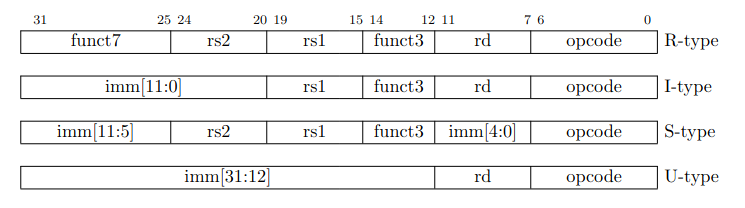
\includegraphics[scale=0.6]{base_isa.png}
  \caption{Base instruction format \cite{waterman2016riscv}}
  \label{fig:base_form}
\end{figure}
Instructions that operate with the PC and conditional instructions such as branches share similar structure with respectively U-type and S-type instructions, in the ISA they are defined as:
\begin{itemize}
  \item \textbf{B-type} or SB-type: Just as in store operations, the rs1 and rs2 addresses are coded in the same position, with the difference that the immediate value has its bits coded in different positions (imm[12] on bit 31, imm[11] on bit 7, imm[10:5] from bit 30 to 25, imm[4:1] from bit 11 to 8). For this type of operation there is no need to change \emph{a\_sel} and \emph{b\_sel}, since, as it will be shown later, the logic unit just operates between registers.
  \item \textbf{J-type} or UJ-type: Jump operations load sums an immediate to the PC and stores the next instruction's PC value. These are coded just as unsigned operations, with the difference being the immediate's bits having different positions (imm[20] on position 31, imm[19:12] from position 19 to 12, imm[11] on bit 20 and imm[10:1] from position 30 to 21).
\end{itemize}
With these definitions, the base ISA extends to this:

\begin{figure}[ht]
  \centering
  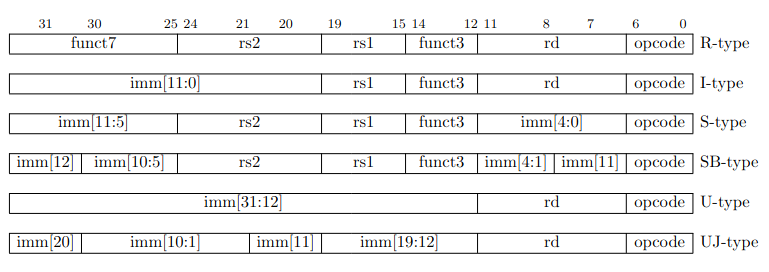
\includegraphics[scale=0.58]{base_isa_2.png}
  \caption{Full 32-bit instruction format \cite{waterman2016riscv}}
  \label{fig:full_form}
\end{figure}
Knowing that the next block can be programmed to use certain parts of the instruction in a certain way, the VHDL code for the ID architecture can be simplified by giving out all the sections of the instruction and letting the Instruction Execute select what specific parts of it are needed.

\subsection{Decoding}
\subsubsection{Reading opcodes for operand selection}
The encoding type of an instruction is not sufficient to detect what operation is actually performed. For example, \emph{LW} and \emph{ADDI} are both I-type instructions but the latter has its result written somewhere in the Register File instead of the Data Memory.
For this reason it is necessary to assess some information segments inside the instruction itself. By looking at Figure \ref{fig:full_form} it is noticeable that there are at most three elements that are descriptive of the content of the instruction and its behavior:
\begin{itemize}
  \item \textbf{opcode}: Unique and present in every instruction, composed by the first 7 bits (starting from the LSB, considering a Little Endian encoding).
  \item \textbf{funct3}: Present in all instructions but U and J -types, made by bit 12 up to 14, necessary for the ALU to select the arithmetic or logic operation to be executed.
  \item \textbf{funct7}: Only for R-type instructions, in the RV32I ISA only one of the seven bits is used.
\end{itemize}
It's obvious that \emph{funct3} and \emph{funct7} do not give information about the identity of the instruction, it is the \emph{opcode} that differentiates the operation and therefore the one that has to be taken into account. The Instruction Set manual [described by Waterman et al. (2016) \cite{waterman2016riscv} page 53 Table 9.1] gives the general opcode map that can help to discriminate instructions: 

\begin{figure}[h!]
  \centering
  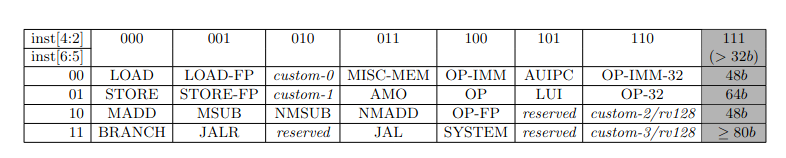
\includegraphics[scale=0.55]{opcodes.png}
  \caption{RISC-V base opcode map \cite{waterman2016riscv}} 
\end{figure}
In a non-superscalar design that does not take into account multiplications, floating-point operations, just implementing \textbf{LOAD}, \textbf{STORE}, \textbf{BRANCH}, \textbf{JALR}, \textbf{JAL}, \textbf{OP} and \textbf{OP-IMM} is sufficient.
The opcode map gives the idea that a decoder can be described with a nested case statement, with an external case structure driven by the last two bits of the opcode, from which is possible to extrapolate what are the operands to be passed to the ALU or Logic Unit, being it the PC, two registers or an immediate and a register.  

\subsubsection{Classification for the Write Back}
The last and most delicate problem that arises when decoding instructions is that they operate in different ways even if they share the same encoding type, for example, ADDI will write the result of the arithmetic operation in a destination register, while LW will have the destination register be a memory location pointed by the result of another arithmetic operation. Also, the interaction with the PC is different even between same-type instructions, hence there is the additional requirement to define in advance a classification method in advance so that the Write Back stage can select what can has to be passed to the Register File and select the next value for the Program Counter. There are three possible cases in which the Write Back accesses the register file: Jumps (since they write back the return address), Loads and arithmetic/logic operations; In addition, the PC can have a new value loaded if, during a branch intruction, the Logic Unit returns a logic high, or during a jump instruction. Otherwise, PC+4 is always returned as next value.
The ID can encode these informations for the next stages as a 5 bit vector, with a one-hot encoding for Arithmetic-Logic Operations, Jump, Load and Store, since store operations can be added as an additional bit that can be used as a write-enable for the Data Memory.

\subsection{Final concept for the ID and simulation}
The finalized concept of the Instruction decode, which follows the block diagram at Figure \ref{fig:ID_BD}, introduces the Register File and a specialized block for decoding, taking as inputs all the IF's outputs (including {pc\_out} and {next\_pc} for sign extension).

As it was done for the Instruction Memory, the Register File was added to the project through the Distributed Memory Generator IP, declared as a dual port RAM with 32 32-bit registers, hence with 5 address bits. The most complex part of this stage, the decoder, is implemented as two nested case statements, with the outer statement using the two most significant bits of the opcode. A snippet is provided at Notes Code \ref{code:ID_decoder}.
By using the same testbench as for the IF and istantiating the ID (Notes Code \ref{code:ID_TB}), by routing the selected instruction and the PC's values, the code is expected to fetch the instruction 0x00000293 (\emph{addi x5 x0 0}, i.e. $x5 = x0 + 0$), decode it and classify it as an operation with an immediate as second operand, hence with \emph{a{\_}sel}=1, \emph{b{\_}sel}=0 and \emph{op{\_}class}=00010, in fact:

\begin{figure}[h!]
  \centering
  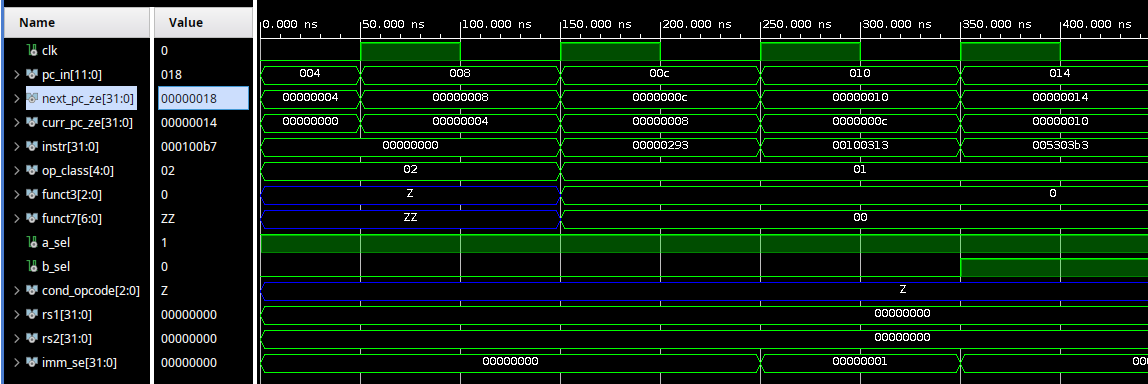
\includegraphics[scale=0.37]{ID_sim.png}
\end{figure}

One particular oservation that could be made is that the Decoder, at any point where the IM returns an empty instruction, i.e. with its hexadecimal value at 0, the decoder is going to report it as a LOAD instruction, with \emph{op{\_}class} = "00010". Of course this doesn't mean the decoder is not working correctly but it is due to the decoder not analyzing the first two bits of the opcode, which in 32-bit architectures should be "11"; For this reason, with all the other bits being at zero, the case statement of the decoder is going to stop at the first case, that is, the case for a LOAD instruction.
\newpage

\section{Basic Instruction Execute}
\begin{figure}[ht]
    \centering
    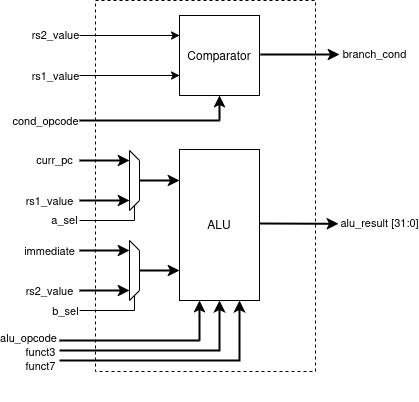
\includegraphics[scale=0.4]{IE_BD.png}
    \caption{A block diagram for the execution stage}
    \label{fig:IE_BD}
\end{figure}

With the information previously decoded from the instruction, the execute stage is responsible for performing the required computation based on the instruction type. This involves selecting the correct operation and applying it to the values stored in the source registers. In a VHDL implementation, the execution stage can be designed as the union of two main blocks: 
\begin{itemize}
\item \textbf{Comparator}: This block evaluates a condition between two 32-bit inputs and returns a boolean result based on the comparison criterion defined by the funct3 field. It is specifically used for branch-type instructions, determining whether a jump in the control flow should occur depending on the result of the comparison.
\item \textbf{Arithmetic-Logic Unit}: This block performs all arithmetic and logical operations, including shift operations. When implementing the ALU, it is important to account for both signed and unsigned computations. To handle this correctly, the inputs to each multiplexer are initially cast as unsigned, ensuring consistency with immediate values, which are inherently unsigned, and then cast appropriately based on the operation being performed.
\end{itemize}
Starting with the ALU, the most complex of them, the first step before implementing its VHDL description is to clearly identify the specific requirements to fetch for each core instruction. This involves selecting the operation the necessary fields to determine the correct arithmetic or logical function and select the correct operators, whether they are represented by registers (including the PC) or immediates. As said earlier, some of them can be distinguished for both the presence of \emph{funct3} (bit 14 to 12) and \emph{funct7}, when dealing with R-type encoding, or just \emph{funct3}. As specified in the base RV32I manual, the univocal codes for the basic core instructions are listed in table \ref{table:core_instr}. It is noticeable that, uniquely in RV32I architectures, the actual purpose of \emph{funct7} is to switch between addition and substraction, since they are encoded as "000", or between logic and arithmetic right shift (i.e SRA and SRL as shown in the table). A simple solution could be editing the behavior of the decoder to onlytake the sixth bit of \emph{funct7} into account and have all subtractions encoded as "010", as it would happen for SLT, and similarly for SRL and SRA. This solution would remove the necessity for \emph{funct7} and shrink the necessary opcode for the ALU to 3 bits. However, that portion of the instruction, seemingly unnecessary for RV32I, comes useful when implementing floating-point instructions and multiplications, hence the most flexible solution, however complex, is to make the decoder return \emph{funct7} and have the ALU taking it into account when switch between operations.
With this in mind now the decoder can be edited to return \emph{funct7} when treating opcodes mapped as OP, and some instances of OP-IMM when treating shifts.With this being said, it is decided that the ALU can switch operation by taking into account, in order of importance: the instruction class, \emph{funct3} and, to maintain flexibility for future modifications, \emph{funct7}.
If the ALU can be defined as a big case statement as for the decoder, Table \ref{table:core_instr} may help to simplify the code, in fact some observations can be already made:
\begin{enumerate}
\item Many instructions expect the ALU to perform an addition, thus if the architecture of the block is written as a case statement, \emph{the addition can be performed if no other case applies}.
\item All load and store operations require \emph{funct3} to be used later during WriteBack stage because they may operate with less than 32 bits, thus it can be useful to \emph{pass it down to the latest stages of the datapath}.
\item Shift operations using immediates are encoded as I-type but they just need five bits indicated as \emph{shamt} (shift amount), for shifting more than 32-bits would not make any sense. While this does not affect SLLI and SRLI, the presence of \emph{funct7} rises a problem with SRAI. \emph{Shifts with immediates need to filter part of the second operand}.
\end{enumerate}
The code for the ALU will thus check the operation class, funct3 and funct7 in the latter sequence. Source code \ref{code:IE_ALU} shows a VHDL implementation that follows said constraints.\\
Branches only require a comparison and just need a single signal to indicate whether or not a jump can happen. From the RV32I instruction table, the remaining core instructions  to implement are indicated in Table \ref{table:core_instr} as BRANCH class instrutions. As it has been for the ALU, the table leads us to a case statement, much simpler than before due to just having to look at \emph{funct3}; A much more self-explanatory architecture can be seen in Source Code \ref{code:IE_comparator}.\\
Finally, the IE (Shown as Source Code \ref{code:IE_code}, much easier to visualize in Figure \ref{fig:IE_BD}) can be "assembled" by routing inputs and outputs of each block, and by also coding multiplexers for the operand selection:

\begin{minted}[fontsize=\footnotesize]{vhdl}
alu_mux_a   <= rs1 when a_sel = '1' else curr_pc;
alu_mux_b   <= rs2 when b_sel = '1' else imm_se;
\end{minted}

\subsection{Simulation}

\begin{figure}[ht]
    \centering
    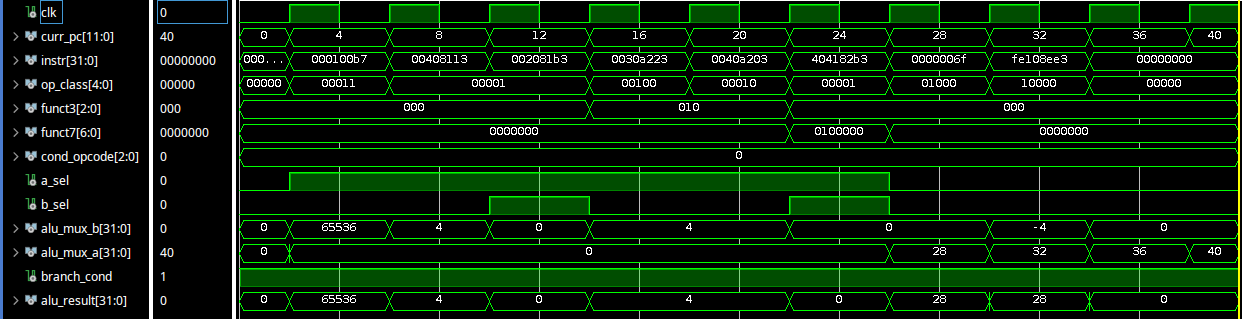
\includegraphics[scale=0.36]{IE_sim.png}
    \caption{Complete IE simulation}
    \label{fig:IE_sim}
\end{figure}

The testbench, following the step-by-step assembly of the whole datapath proposed in the ID section, can be built using a copy of the earlier code with the IE as an addition (Source Code \ref{code:IE_TB}).\\
Now when running a behavioral simulation the following events are expected to happen to be sure that the design is working properly: the first instruction is going to be encoded with \emph{op{\_}class} = "000110", while setting \emph{a{\_}sel} and pulling down \emph{b{\_}sel}, leaving \emph{alu{\_}result} = 65536, because LUI operation imply that the immediate operand is shifted by 16 bits to the left, thus multiplying it by $2^{15}$; The second one should sum the previous result with 4 and the folowing addition should return a 0, since the accessed register cannot yet be written; The following load, store and jump instructions should be performing additions, easy to notice from the ALU's output, which in case of SW and LW, should just return the immediate 4 summed to the registers that are still limited to store just zeroes, while jumps and branches sum the current PC's value to their orresponding immediate value (in Figure \ref{fig:IE_sim}).The subtraction is easily noticed by the fact that it represent the only one that changes \emph{funct7} and the last one should have the comparator set its only output:\\



\section{Data Memory, Write Back and Structural Hazards}
\subsection{Data Memory}
\begin{figure}[!ht]
    \centering
    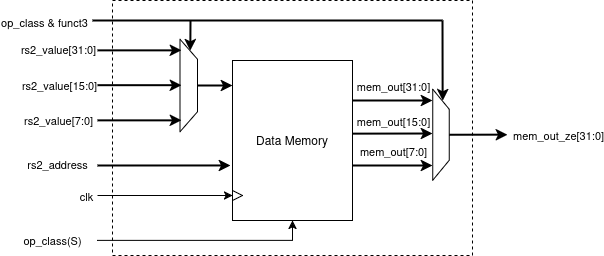
\includegraphics[scale = 0.45]{MEM_BD.png}
    \caption{DM interface block diagram}
    \label{fig:DM_BD}
\end{figure}

The final pieces that remain to be designed are the one that manages the Data Memory, and decides when to write, and the stage which, depending on the operation type, selects what to return as new value for the PC and what to store in the destination register, i.e the Write Back.\\
The Data Memory will instantiated as a 16KB single port RAM and separated from the rest, forming a 5-stage datapath when it is going to be pipelined. In 4-stages architecture it would be instead included in the same block, reducing the overall size of the processor, reducing power consumption, due to the presence of one less register, but at the cost of a reduced throughput.\\
The Table \ref{table:core_instr} indicates that there are many ways to perform L/S instruction and not only 32-bit vectors are handled. In fact some of them could manage just bytes or half-words, leaving some other options to be managed when executing these instructions. This discrimination cannot be performed by the ALU nor the Decoder, but it is easy to implement as interface for the Data Memory.
To be more specific, another case statement can be deployed to select filter the input and output of and from the memory, leaving the discrimination to both \emph{op{\_}class}, to see if an L/S operation is being performed, and \emph{funct3} to classify if the latter is working with bytes, half-words or words.

\subsection{Write Back}
\begin{figure}[!ht]
    \centering
    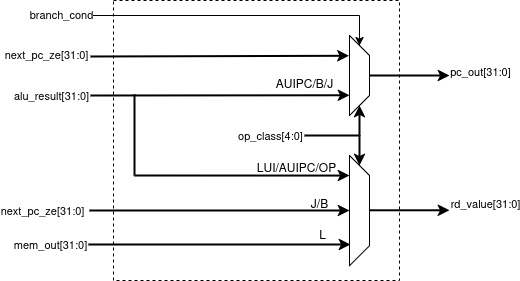
\includegraphics[scale = 0.45]{WB_BD.png}
    \caption{Write Back block diagram}
    \label{fig:WB_BD}
\end{figure}

The final step of execution, where the destination register and the program counter are written, needs a selector to decide what has to be overwritten and where; In the case of the PC two options can be identified: PC + 4 or the result from the ALU, which happens in case of a jump, a true condition from a branch or AUIPC. The destination register instead can be: the output of the ALU for classes OP, LUI, UIPC, PC + 4 for jumps and branches (when a logic high is returned, otherwise a high impedance output can be returned) or the output from the data memory. Source Code \ref{code:WB_code} shows again a case statement enclosed in an input-sensitive process, that is, a simple combinatory network.

\subsection{Simulation and final consideration}
With all the code prepared, the final simulation of the unpipelined datapath can be performed; Leaving the load-enable of the PC high, for there is no need to stall the execution for now, it is noticeable that the overall behavior corresponds to what is expected from it, although with a small concerning bug:

\begin{figure}[!ht]
    \centering
    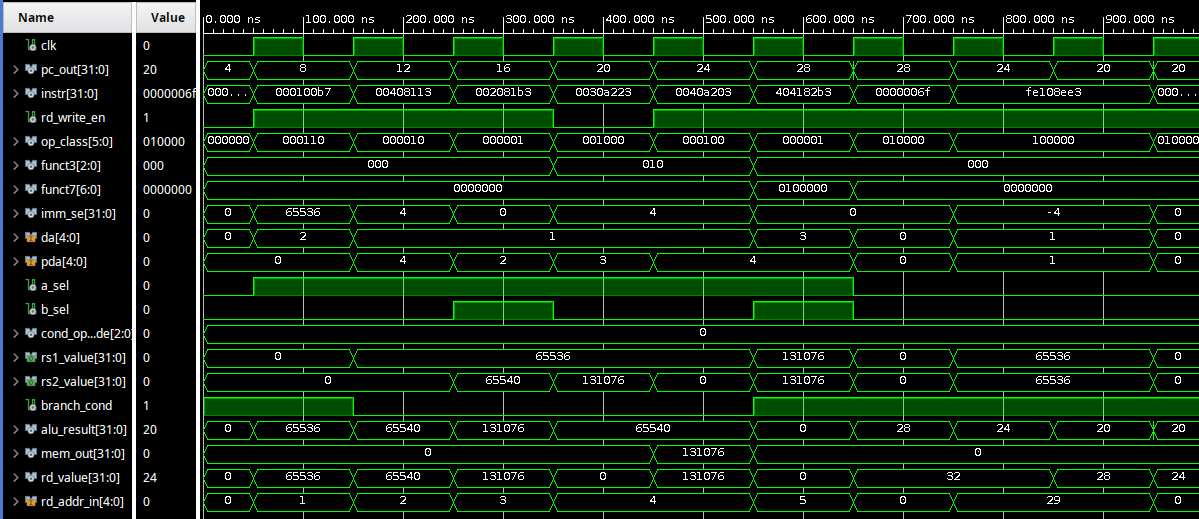
\includegraphics[scale = 0.36]{WB_sim.png}
    \caption{Complete simulation if the unpipelined datapath}
    \label{fig:WB_sim}
\end{figure}

Now L/S operations can effectively interact with the memory, although not each one of them has been tested. Also jumps and branches, with the output value for the PC being routed back to its original register, can move between instructions without problems.\\
A the very end of this basic implementation there are more some considerations to be made. For example x0 \emph{must not} be writable, instead all bits should be hardwired to a logic low, if not possible, then every attempt to write onto that must be ignored.\\
Another thing to observe from the code is that the multiplexer which selects between \emph{rs1} and \emph{rd}, at the end of the cycle will be left to '1', but since the architecture hasn't yet been pipelined, at the end of the operation the destination register cannot be overwritten, because the register file is only read and written during the rising edge of the clock, also during the next instruction, the resource has to be kept free. This is the first \emph{structural hazard} that this architecture is facing, leaving the only option to either stall the datapath for an amount of time after the execution cycle has terminated or implementing a pipeline, that is, having the processes of every stage sensitive to the rising edge of the clock instead of the inputs, meaning that every output is refreshed at that edge, as it would be expected by a register.

\chapter{Developing the Architecture}

\section{Pipeline}
\begin{figure}[!ht]
    \centering
    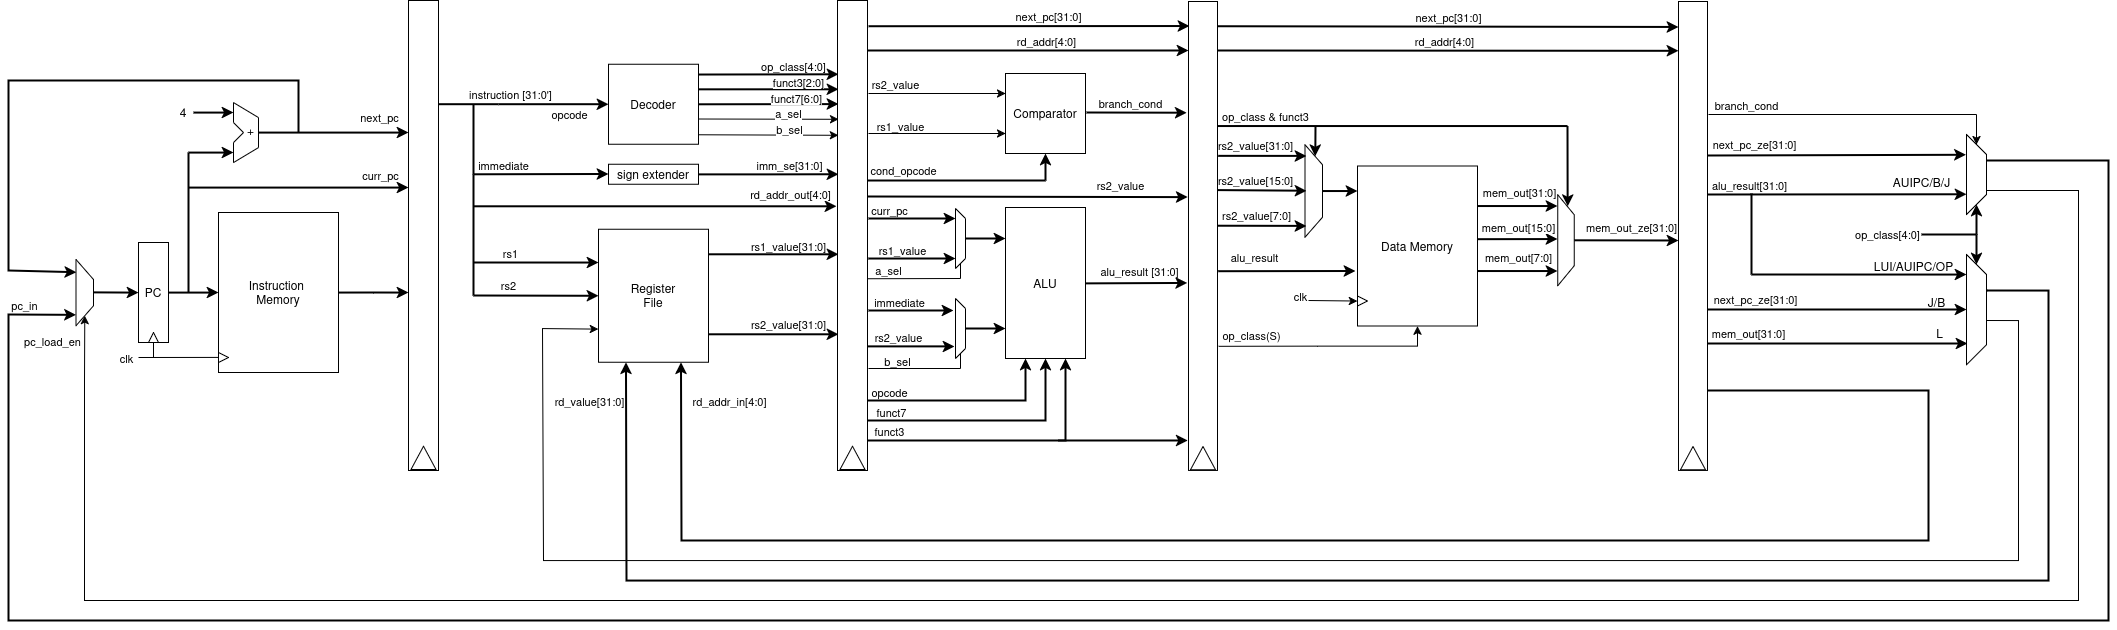
\includegraphics[scale = 0.2]{datapath_pipelined.png}
    \caption{An example of pipelined RISC-V architecture}
    \label{fig:DP_PPL}
\end{figure}

As mentioned earlier, having the processes sensitive to the rising edge of the clock, and having it update output signals after the end is the VHDL equivalent to registers, for example, supposing an input \emph{pc{\_}in} and an output \emph{pc{\_}out}:  

\begin{minted}[fontsize=\footnotesize]{vhdl}
architecture Behavioral of Example is
    signal pc_reg : std_logic_vector(11 downto 0);
begin
process(clk)
    begin
        if rising_edge(clk) then
            pc_reg <= pc_in;
        end if;
    end process;
    pc_out  <= pc_reg;
end Behavioral;
\end{minted}

A process in VHDL executes a routine whenever any signal in the sensitivity list changes, meaning that whatever the routine is, its output is not available until the sensitive inputs change. In the example above \emph{pc{\_}reg} changes only when a rising edge of the clock approaches, thus keeping the output still for the whole clock cycle; The same concept can be applied to all the blocks that compose the architecture, by having all processes clock-sensitive, some kind of pipeline can be naturally implemented.\\
This method, however convenient, does not take into account the signals that are used in multiple process, for example, if \emph{funct3} is passed directly to the DM stage, with \emph{op{\_}class} commanded by a different instruction, the DM could wrongly load or store the result of the original operation.\\
Both for this reason and for not having to change the whole code and thus maintaining clarity over the project's code, the inter-stage registers will be programmed as separate blocks in VHDL. Before starting to code, it is imperative to identify which signals are the ones that need to be passed down and the ones that are not useful anymore. 
From simple analysys of the code, Table \ref{table:signals_pipeline} lists all the outputs expected at the boundary of each stage, indicated as the union of the names of the two stages that the boundary shares.

\begin{table}[ht]
\begin{center}
\begin{tabular}{|c|c|c|c|c|}
    \hline
    IF/ID & ID/IE & IE/DM & DM/WB & WB \\
    \hline
    curr{\_}pc  & curr{\_}pc        & curr{\_}pc        & next{\_}pc        & pc{\_}out \\
    next{\_}pc  & next{\_}pc        & next{\_}pc        & mem{\_}out        & rd{\_}value \\
    instr       & op{\_}class       & op{\_}class       & branch{\_}cond    & pc{\_}load{\_}en\\
                & funct3            & funct3            & alu{\_}result     & mem{\_}we\\
                & funct7            & alu{\_}result     & rd{\_}addr        & rd{\_}addr\\
                & a{\_}sel          & branch{\_}cond    & op{\_}class       & \\
                & b{\_}sel          & rs2{\_}value      &                   & \\
                & imm{\_}se         & rd{\_}addr        &                   & \\
                & rs1{\_}value      &                   &                   & \\
                & rs2{\_}value      &                   &                   & \\
                & rd{\_}addr        &                   &                   & \\
                & cond{\_}opcode    &                   &                   & \\
    \hline
\end{tabular}
\caption{List of input signals for each register}
\label{table:signals_pipeline}
\end{center}
\end{table}

Once that each register is described, not timing requirements for setting the load enable for both destination register and Program Counter is needed, since the change in the IF's input can be updated every clock cycle without any risk of glitching due to the simulation not taking into account the delay of each stage. 
Before setting up the Structural definition of the datapath, including registers and major blocks, the IF stage must be edited to increment the PC before the first register, otherwise PC+4 would instead be returned by the WB, 4 clock cycle after the instruction is first withdrawed from the IM. With this being said, WB will return a value for the PC only during jumps and branches, while the IF will select between PC+4 and the returning value from WB.

\begin{figure}[!ht]
    \centering
    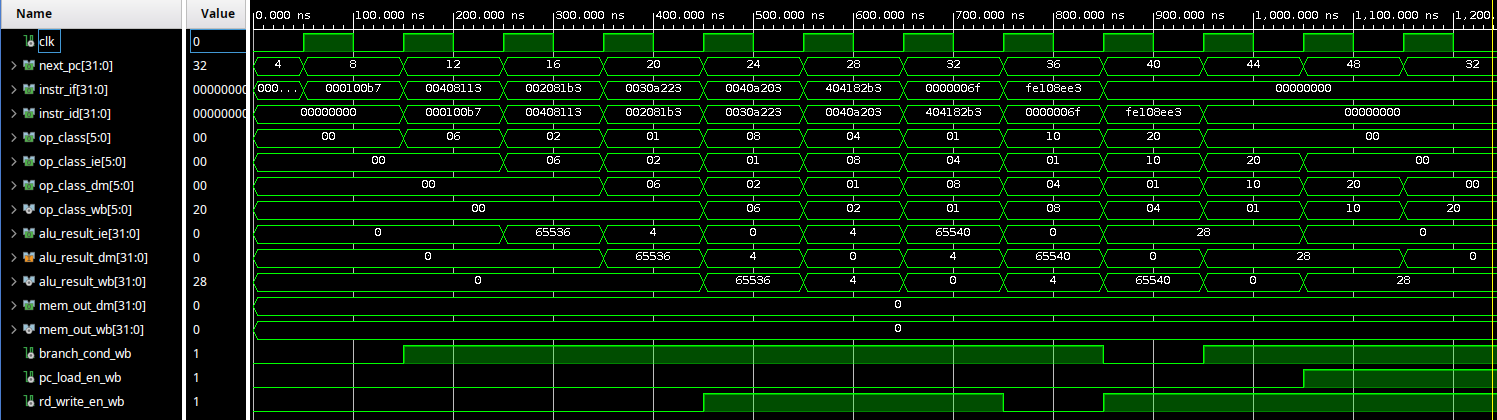
\includegraphics[scale = 0.3]{DPPPL_sim.png}
    \caption{Datapath simulation with pipeline}
    \label{fig:DPPPL_sim}
\end{figure}

Now the processor can execute a part of the instruction in a clock cycle, allowing for higher clock speeds, yet this improvement creates some bugs, one of which can be directly observed from Figure \ref{fig:DPPPL_sim}; In fact, right after the second instruction reaches the execution stage, the \emph{addi} retrieves a 0 instead of 65535 as content of x1, as happens in Figure \ref{fig:WB_sim} where the instruction returns 65540 as a result.
Also, in case of jumps and branches, the correct value for the Program Counter is updated after one clock cycles while the previous instructions still get executed. In addition, since x1 is updated only after 5 clock cycles, the store and load instrucction will operate with different addresses.
While the architecture is now completed, it misses some important features that solve these types of hazards and therefore ensure correct program execution; Thus it becomes essential to implement mechanisms that can handle such hazards to preserve instruction accuracy and consistency while maintaining the performance of a pipelined architecture.  

\let\cleardoublepage\clearpage

\chapter{Appendices}
\section{Appendix A: Instruction Tables}

\begin{table}[ht]
    \begin{center}
        \begin{tabular}{|c|c|c|c|c|}
            \hline
            class & funct7 & funct3 & instruction & operation \\
            \hline
            \multirow{10}{*}{OP} & 0000000 & 000 & ADD & addition\\
            & 0100000 & 000 & SUB & subtraction\\
            & 0000000 & 001 & SLL & left logic shift\\
            & 0000000 & 010 & SLT & set if less than\\
            & 0000000 & 011 & SLTU & set if less than unsigned\\
            & 0000000 & 100 & XOR & bit-wise EXOR\\
            & 0000000 & 101 & SRL & right logic shift\\
            & 0100000 & 101 & SRA & right arithmetic shift\\
            & 0000000 & 110 & OR & bit-wise OR\\
            & 0000000 & 111 & AND & bit-wise AND\\
            \hline
            \multirow{9}{*}{OP-IMM} & - & 000 & ADDI & addition\\
            & 0000000 & 001 & SLLI & left logic shift\\
            & - & 010 & SLTI & set if less than\\
            & - & 011 & SLTIU & set if less than unsigned\\
            & - & 100 & XORI & bit-wise EXOR\\
            & 0000000 & 101 & SRLI & right logic shift\\
            & 0100000 & 101 & SRAI & right arithmetic shift\\
            & - & 110 & ORI & bit-wise OR\\
            & - & 111 & ANDI & bit-wise AND\\
            \hline
            \multirow{3}{*}{STORE} & - & 000 & SB & addition\\
            & - & 001 & SH & addition\\
            & - & 010 & SW & addition\\
            \hline
            \multirow{5}{*}{LOAD} & - & 000 & LB & addition\\
            & - & 001 & LH & addition\\
            & - & 010 & LW & addition\\
            & - & 100 & LBU & addition\\
            & - & 101 & LHU & addition\\
            \hline
            JALR & - & 000 & JALR & addition\\
            \hline
            JAL & - & - & JAL & addition\\
            \hline
            LUI & - & - & LUI (pseudo instruction LI) & addition\\
            \hline
            AUIPC & - & - & AUIPC & addition\\
            \hline
            \multirow{6}{*}{BRANCH} & - & 000 & BEQ & branch if equal\\
            & - & 001 & BNE & branch if not equal\\
            & - & 100 & BLT & branch if lower than\\
            & - & 101 & BGE & branch if greater or equal\\
            & - & 110 & BLTU & branch if lower than unsigned\\
            & - & 111 & BGEU & branch if greater or equal unsigned\\
            \hline
        \end{tabular}
        \caption{RV32I core instructions}
        \label{table:core_instr}
    \end{center}
\end{table}

\section{Appendix B: Code segments of unpipelined datapath}

\subsection{Instruction Fetch [RV32I]}

\subsubsection{Base architecture}
\begin{code}
\captionof{listing}{Architecure of the Instruction Fetch}
\label{code:IF_code}   
\inputminted[fontsize=\footnotesize]{vhdl}{\srcfolder instr_fetch.vhd}
\end{code}
\newpage


\subsubsection{Testbench}
\begin{code}
\captionof{listing}{first Instruction Fetch testbench}
\label{code:IF_TB}
\inputminted[fontsize=\footnotesize]{vhdl}{\simfolder IF_testbench.vhd}
\end{code}
\newpage

\subsubsection{Instruction Decode [RV32I]}
\begin{code}
\captionof{listing}{Architecure of the Instruction Fetch}
\label{code:ID_code}  
\inputminted[fontsize=\footnotesize]{vhdl}{\srcfolder instr_decode.vhd}
\end{code}

\subsubsection{Decoder}
\begin{code}
\captionof{listing}{Decoder fully implementing RV32I instructions}
\label{code:ID_decoder}  
\inputminted[fontsize=\footnotesize]{vhdl}{\srcfolder decoder.vhd}
\end{code}

\subsubsection{Register File}
\begin{code}
\captionof{listing}{Simple 32 bits Register File}
\label{code:reg_file}  
\inputminted[fontsize=\footnotesize]{vhdl}{\srcfolder register_file.vhd}
\end{code}

\subsubsection{Testbench}
\begin{code}
\captionof{listing}{Instruction Decode Testbench}
\label{code:ID_TB}  
\inputminted[fontsize=\footnotesize]{vhdl}{\simfolder ID_testbench.vhd}
\end{code}
\newpage


\subsection{Instruction Execute [RV32I]}
\subsubsection{Architecture}
\begin{code}
\captionof{listing}{Architecture of Instruction Execute}
\label{code:IE_code}  
\inputminted[fontsize=\footnotesize]{vhdl}{\srcfolder instr_exec.vhd}
\end{code}

\subsubsection{ALU}
\begin{code}
\captionof{listing}{ALU}
\label{code:IE_ALU}  
\inputminted[fontsize=\footnotesize]{vhdl}{\srcfolder ALU.vhd}
\end{code}
\newpage


\subsubsection{Comparator}
\begin{code}
\captionof{listing}{Comparator}
\label{code:IE_comparator}  
\inputminted[fontsize=\footnotesize]{vhdl}{\srcfolder comparator.vhd}
\end{code}
\newpage


\subsubsection{Testbench}
\begin{code}
\captionof{listing}{Instruction Execute Testbench}
\label{code:IE_TB}  
\inputminted[fontsize=\footnotesize]{vhdl}{\simfolder IE_testbench.vhd}
\end{code}
\newpage


\subsection{Data Memory [RV32I]}
\begin{code}
\captionof{listing}{Data Memory stage}
\label{code:DM_code}  
\inputminted[fontsize=\footnotesize]{vhdl}{\srcfolder data_memory.vhd}
\end{code}


\subsection{WriteBack [RV32I]}
\begin{code}
\captionof{listing}{Write Back stage}
\label{code:WB_code}  
\inputminted[fontsize=\footnotesize]{vhdl}{\srcfolder write_back.vhd}
\end{code}

\subsection{Unpipelined Datapath Simulation}
\begin{code}
\captionof{listing}{Testbench with all components of the RV32I datapath}
\label{code:DPP_TB}  
\inputminted[fontsize=\footnotesize]{vhdl}{\simfolder WB_testbench.vhd}
\end{code}
\newpage

\section{Appendix C: Code segments of the finalized datapath}

\subsection{Final Instruction Fetch entity description}
\begin{code}
\captionof{listing}{Instruction Fetch implemented for a pipelined architecture}
\label{code:IF_PPLND}  
\inputminted[fontsize=\footnotesize]{vhdl}{\srcfolder instr_fetch_pipeline.vhd}
\end{code}

\subsection{Final Instruction Decode entity description}
\begin{code}
\captionof{listing}{Instruction Decode implemented for a pipelined architecture}
\label{code:ID_PPLND}  
\inputminted[fontsize=\footnotesize]{vhdl}{\srcfolder instr_decode_pipeline.vhd}
\end{code}

\subsection{Final Instruction Execute entity description}
\begin{code}
\captionof{listing}{Instruction Execute implemented for a pipelined architecture}
\label{code:IE_PPLND}  
\inputminted[fontsize=\footnotesize]{vhdl}{\srcfolder instr_exec_pipeline.vhd}
\end{code}

\subsection{Final Data Memory stage entity description}
\begin{code}
\captionof{listing}{Data Memory implemented for a pipelined architecture}
\label{code:DM_PPLND}  
\inputminted[fontsize=\footnotesize]{vhdl}{\srcfolder data_memory_pipeline.vhd}
\end{code}

\subsection{IF/ID register}
\begin{code}
\captionof{listing}{IF/ID register}
\label{code:IF_ID}  
\inputminted[fontsize=\footnotesize]{vhdl}{\srcfolder IF_ID.vhd}
\end{code}

\subsection{ID/IE register}
\begin{code}
\captionof{listing}{ID/IE register}
\label{code:ID_IE}  
\inputminted[fontsize=\footnotesize]{vhdl}{\srcfolder ID_IE.vhd}
\end{code}

\subsection{IE/DM register}
\begin{code}
\captionof{listing}{IE/DM register}
\label{code:IE_DM}  
\inputminted[fontsize=\footnotesize]{vhdl}{\srcfolder IE_DM.vhd}
\end{code}

\subsection{DM/WB register}
\begin{code}
\captionof{listing}{DM/WB register}
\label{code:DM_WB}  
\inputminted[fontsize=\footnotesize]{vhdl}{\srcfolder DM_WB.vhd}
\end{code}

\subsection{Pipelined architecture (Structural definition)}
\begin{code}
\captionof{listing}{Structural definition of a pipelined datapath}
\label{code:DTPTH_pipelined}  
\inputminted[fontsize=\footnotesize]{vhdl}{\srcfolder datapath.vhd}
\end{code}


\section{Appendix D: Testing Block for Nexys 4}

\subsection{Reading from register file and DM}
\begin{code}
\captionof{listing}{Architecture of a register and DM reader with a 7-segments display driver for Nexys 4 DDR}
\label{code:mem_read}  
\inputminted[fontsize=\footnotesize]{vhdl}{\srcfolder memory_reader.vhd}
\end{code}

\bibliographystyle{plain} 
\bibliography{bibliography}

\end{document}